\section{About the Author}

\begin{frame}
  \frametitle{About yours truly}

  \begin{itemize}
    \item Contributor to/Author of many Open Source projects
    \item Member of the GNOME Foundation
    \item Former member of Igalia and Red Hat
    \item Currently at the Data Storage Services group at CERN
    \item http://www.joaquimrocha.com
  \end{itemize}
\end{frame}

%%%%%%%%%%%%%%%%%%%%

\section{Introduction}

%%%%%%%%%%%%%%%%%%%%

\subsection{What's git}

{
\usebackgroundtemplate{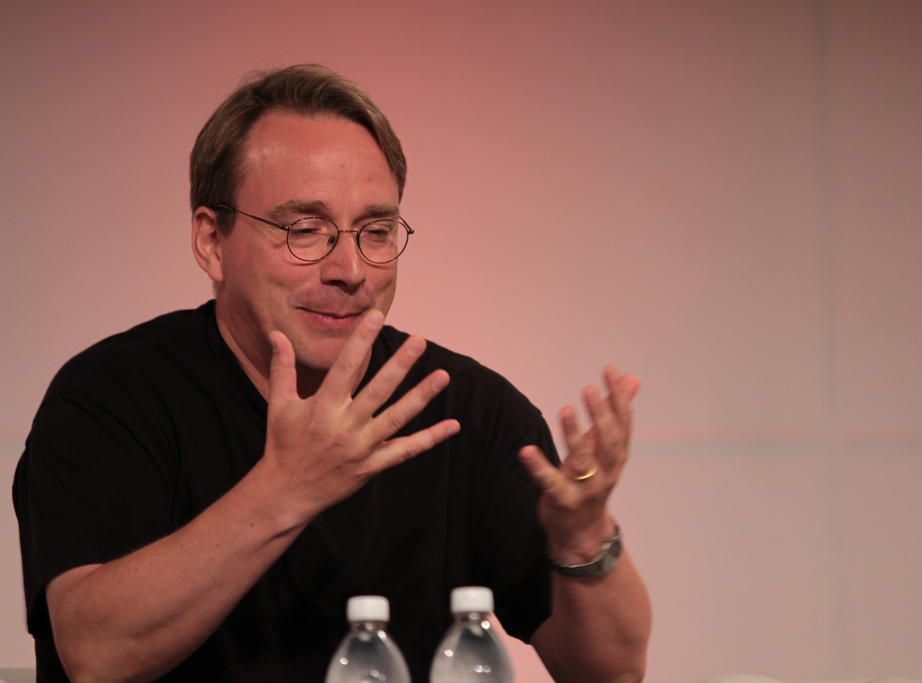
\includegraphics[width=\paperwidth]{images/linus.jpg}}
\begin{frame}[plain]
  \begin{center}
    \vspace{140pt}\color{White}
    \textbf{\textit{``I'm an egotistical bastard, so I name all my projects after myself. First Linux, now git"}\\\vspace{10pt}
    Linus Torvalds}
  \end{center}
\end{frame}
}

%%%%%%%%%%%%%%%%%%%%

\begin{frame}
  \frametitle{\insertsubsection}

  \begin{itemize}
    \item \textbf{Distributed} Version Control System (\textit{DVCS}) \vspacing
    \item Initially written in C by Linus Torvalds\vspacing
    \item Replacement for \textit{BitKeeper} in Linux kernel development \vspacing
    \item Widely used nowadays, both for new and old projects
  \end{itemize}
\end{frame}

%%%%%%%%%%%%%%%%%%%%

\subsubsection{VCS vs DVCS}

\begin{frame}[plain]
%  \frametitle{\insertsubsection}

  \begin{center}
    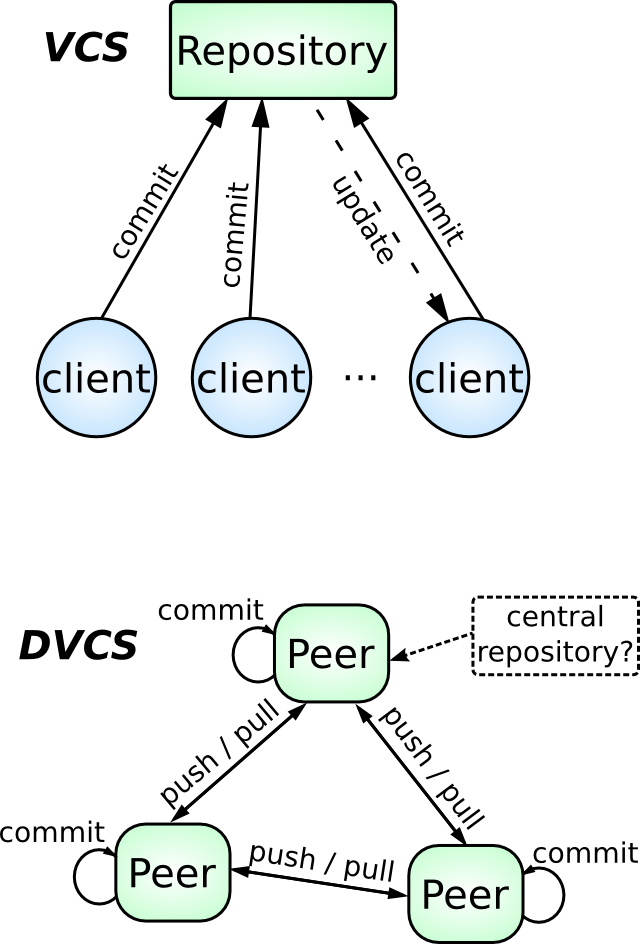
\includegraphics[height=1.0\textheight]{images/vcs-vs-dvcs.png}
  \end{center}
\end{frame}

%%%%%%%%%%%%%%%%%%%%

\subsubsection{Git Layout}

\begin{frame}[plain]
  \frametitle{\insertsubsection}

  \begin{center}
    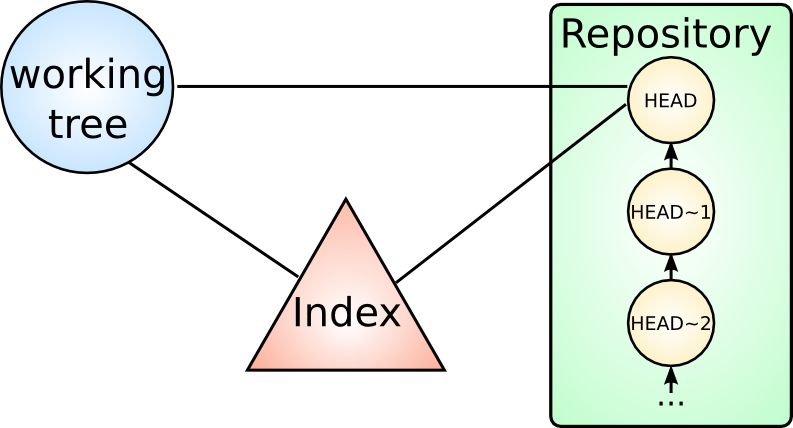
\includegraphics[width=1.0\textwidth]{images/git-layout.png}
  \end{center}
\end{frame}

%%%%%%%%%%%%%%%%%%%%

\subsubsection{Working Tree}

%%%%%%%%%%%%%%%%%%%%

\begin{frame}

  \begin{center}
    
\includegraphics[width=.25\textwidth]{images/git-working-tree.png}\\\vspacing
    \Large{It's the sandbox}
  \end{center}
\end{frame}

%%%%%%%%%%%%%%%%%%%%

\begin{frame}

  \begin{center}
    
\includegraphics[width=.25\textwidth]{images/git-index.png}\\\vspacing
    \Large{Holds the new changes to be commited}
  \end{center}
\end{frame}

%%%%%%%%%%%%%%%%%%%%

\begin{frame}

  \begin{center}
    
\includegraphics[width=.25\textwidth]{images/git-head.png}\\\vspacing
    \Large{Points to the current commit}
  \end{center}
\end{frame}

%%%%%%%%%%%%%%%%%%%%

\begin{frame}[plain]

  \begin{center}
    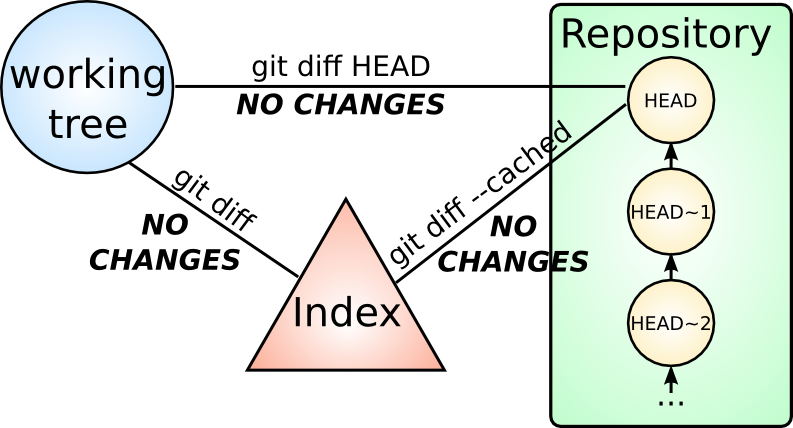
\includegraphics[width=1.0\textwidth]{images/git-diffs.png}
  \end{center}
\end{frame}

%%%%%%%%%%%%%%%%%%%%

\begin{frame}
  \frametitle{Working Tree with Changes}

  \begin{center}
    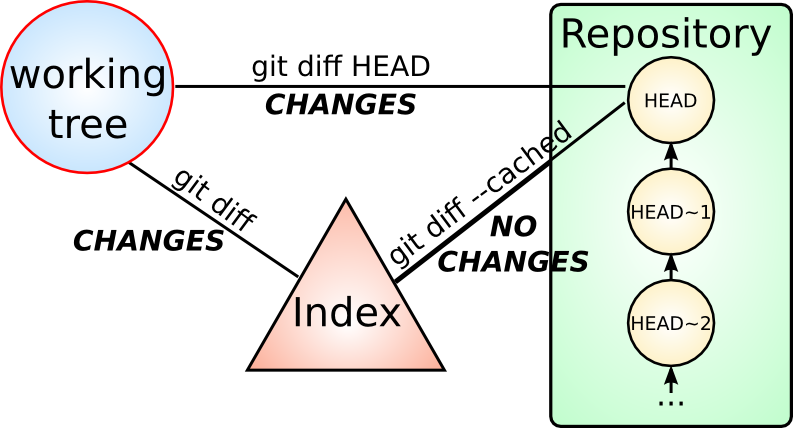
\includegraphics[width=1.0\textwidth]{images/git-diffs-changes.png}
  \end{center}
\end{frame}

%%%%%%%%%%%%%%%%%%%%

\begin{frame}

  \begin{center}
    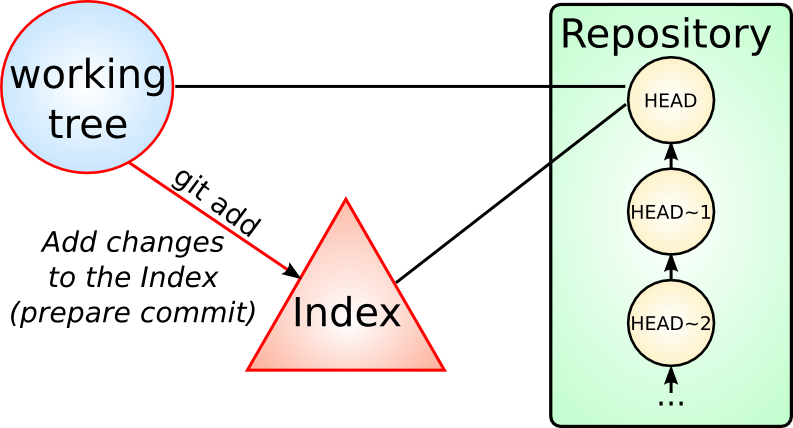
\includegraphics[width=1.0\textwidth]{images/git-add.png}
  \end{center}
\end{frame}

%%%%%%%%%%%%%%%%%%%%

\begin{frame}
  \frametitle{Index with Changes}

  \begin{center}
    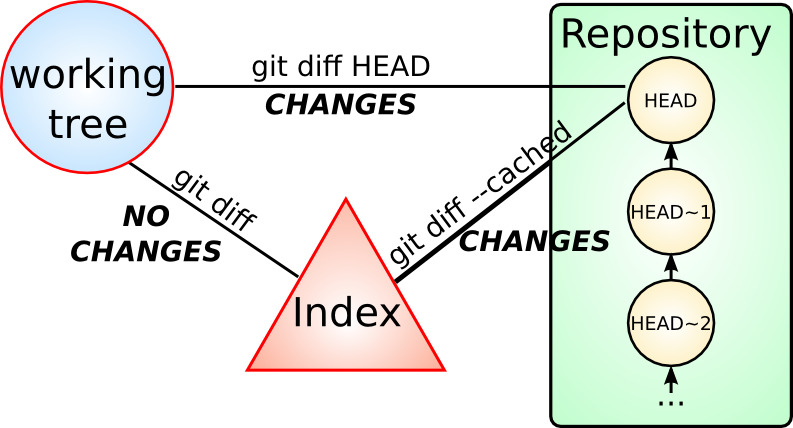
\includegraphics[width=1.0\textwidth]{images/git-diff-cached-changes.png}
  \end{center}
\end{frame}

%%%%%%%%%%%%%%%%%%%%

\begin{frame}
%  \frametitle{\insertsection}

  \textbf{Typical beginners' workflow with git:\\}

  \begin{enumerate}
    \item \texttt{git clone URL} or \texttt{git init .}
    \item \textit{Do stuff...}
    \item \texttt{git add -{}-all} or \texttt{git add FILE}
    \item \texttt{git commit -m ``Update"} \textit{[or another bad description]}
    \item \texttt{git push}
  \end{enumerate}
\end{frame}

%%%%%%%%%%%%%%%%%%%%

{
\usebackgroundtemplate{
\includegraphics[width=\paperwidth]{images/kid-eating.jpg}}
\begin{frame}[plain]
\end{frame}
}

%%%%%%%%%%%%%%%%%%%%

\section{Best Practices}

\begin{frame}[plain]

  \begin{center}
    \Huge{\textbf{\insertsection}}
  \end{center}

\end{frame}

%%%%%%%%%%%%%%%%%%%%

\subsection{Adding Files}

\begin{frame}

  \begin{center}
    \Huge{\textbf{\insertsubsection}}
  \end{center}

\end{frame}

%%%%%%%%%%%%%%%%%%%%

\begin{frame}
  \frametitle{\insertsubsection}

  \textbf{Do NOT}:
  \begin{itemize}
    \item \texttt{git add *}
    \item \texttt{git add .}
    \item \texttt{git add -{}-all}\\
    \item \texttt{git add -u .}\\
    ... and unless you're adding a new (unknown to index) file:
    \item \texttt{git add FILE\_PATH}
  \end{itemize}
\end{frame}

%%%%%%%%%%%%%%%%%%%%

\begin{frame}
  \frametitle{\insertsubsection}

  Please \textbf{Do}:\vspacing
  \begin{center}
    \Huge{git add -{}-patch}
  \end{center}
\end{frame}

%%%%%%%%%%%%%%%%%%%%

\begin{frame}
  \frametitle{\insertsubsection}

  \center{\texttt{git add -{}-patch} or \texttt{git add -p}}\vspace{20pt}\\

  \begin{itemize}
    \item asks you which chunks of code should be added and how!
    \item means you review your code before adding it!
    \item helps you create atomic commits!
  \end{itemize}
\end{frame}

%%%%%%%%%%%%%%%%%%%%

\begin{frame}[fragile]
  \frametitle{\insertsubsection: Example}

  \begin{small}
\begin{verbatim}
[...]

   if (delegateAuthLibPath)
     loadDelegateAuthLib(delegateAuthLibPath);
+
+  fprintf(stderr, "WHY THE HELL DOESN'T THIS WORK!!");
 }

 AuthChangeFsUid::~AuthChangeFsUid()
Stage this hunk \[y,n,q,a,d,/,j,J,g,e,?\]?
\end{verbatim}
  \end{small}

\end{frame}

%%%%%%%%%%%%%%%%%%%%

\subsection{Committing}

\begin{frame}

  \begin{center}
    \textbf{\Huge{\insertsubsection}}
  \end{center}

\end{frame}

%%%%%%%%%%%%%%%%%%%%

\begin{frame}
  \frametitle{\insertsubsection}

  \begin{center}
    \begin{itemize}
      \item Do \textbf{atomic commits}!
      \item Write useful, descriptive commit messages!
      \item Don't be affraid of commiting (you'll see why later)!
    \end{itemize}
  \end{center}

\end{frame}

%%%%%%%%%%%%%%%%%%%%

\subsubsection{Atomic Commits}

{
\usebackgroundtemplate{
\includegraphics[width=\paperwidth]{images/sherlock-monkey.jpg}}
\begin{frame}[plain]
  \frametitle{\insertsubsubsection}

  \vspace*{.6\textheight}
  \begin{center}\color{White}
    \Large{Sherlock was investigating why the new version of his team's software didn't work...}
  \end{center}

\end{frame}
}

%%%%%%%%%%%%%%%%%%%%

\begin{frame}[fragile]
  \frametitle{\insertsubsubsection}

    He quickly looked at his favorite git UI (which uses \texttt{git log -{}-oneline} log) for clues...\\\vspacing

  \begin{small}
\begin{verbatim}
1d60cd2 Update for 1.5.0
817ee03 Innocent stuff...
8341828 Innocent stuff #1...
afee627 Innocent stuff #2...
d4c29b7 Innocent stuff #3...
c3bdb6d Innocent stuff #4...
a3e8c35 Innocent stuff #5...
fd9f14b Innocent stuff #6...
da8a2cf Innocent stuff #7...
c2debc0 Innocent stuff #8...
283293c Innocent stuff #9...
...
\end{verbatim}
  \end{small}

\end{frame}

%%%%%%%%%%%%%%%%%%%%

\begin{frame}
  \frametitle{\insertsubsubsection}

  \begin{center}
    Not finding anything suspicious in the log, Sherlock starts a bisect in order to find the problem!\\\vspacing
    With all the compiling and testing, he spends hours in the bisect before finding the culprit:\\\vspacing
    \Large{1d60cd2 Update for 1.5.0}
  \end{center}

\end{frame}

%%%%%%%%%%%%%%%%%%%%

\begin{frame}[fragile]
  \frametitle{\insertsubsubsection}

  \begin{center}
    Sherlock finds out the commit has more to it than meets the eye...\\\vspacing
  \end{center}

\begin{verbatim}
commit 1d60cd23c6597f1d11288644691b582bd531e704
Author: Moriarty <moriarty.indeed@evil-r-us.co.uk>
Date: Thu Jun 6 18:06:06 2013 +0100

    Update for 1.5.0

    Evil stuff because I can!
    More evil stuff because I can!
    ...
\end{verbatim}

\end{frame}

%%%%%%%%%%%%%%%%%%%%

{
\usebackgroundtemplate{
\includegraphics[width=\paperwidth]{images/sherlock-monkey-evil.jpg}}
\begin{frame}[plain]
  % PICTURE OF SHERLOCK HOLMES

  \begin{center}
    \vspace*{.7\textheight}
    \textbf{\Huge{\color{White}Always write atomic commits!}}
  \end{center}
\end{frame}
}

%%%%%%%%%%%%%%%%%%%%

\subsection{Write useful commit messages}

\begin{frame}
  \begin{center}
    \Huge{\textbf{\insertsubsection}}
  \end{center}
\end{frame}

%%%%%%%%%%%%%%%%%%%%

\begin{frame}[fragile]
  \frametitle{\insertsubsection}

  \textbf{A good commit message:}\\
  \begin{footnotesize}
\begin{verbatim}
Imperative tense summary, <= 50 chars

When necessary, more details can come here, until 72 chars
each line.
A reference to a bug tracker issue can be added as well:

http://bugtracker.earth/issue/1985
\end{verbatim}
  \end{footnotesize}

\end{frame}

%%%%%%%%%%%%%%%%%%%%

\begin{frame}[fragile]
  \frametitle{\insertsubsection}

  \begin{block}{\color{Red}Bad}

    \begin{footnotesize}
\begin{verbatim}
fixes a crash
\end{verbatim}
    \end{footnotesize}

  \end{block}

  \begin{block}{\color{Red}Awful}

    \begin{footnotesize}
\begin{verbatim}
fix
\end{verbatim}
    \end{footnotesize}

  \end{block}

\vspace{20pt}
  \begin{block}{\color{LimeGreen}Good}

    \begin{footnotesize}
\begin{verbatim}
Fix crash when performing update

The issue was being caused when the Updater was called
and a network connection that had been used before
is no longer available.

https://sherlocksbugtracker.co.uk/issue/1985
\end{verbatim}
    \end{footnotesize}
  \end{block}

\end{frame}

%%%%%%%%%%%%%%%%%%%%

\subsection{Know How to Use References}

\begin{frame}
  \begin{center}
    \Huge{\textbf{\insertsubsection}}
  \end{center}
\end{frame}

%%%%%%%%%%%%%%%%%%%%

\begin{frame}[fragile]
  \frametitle{\insertsubsection}

  \textbf{Specific References:}\vspacing
  \begin{itemize}
    \item The current commit: \textit{HEAD}
    \item A hash from some commit, e.g.:\\
      \textit{d3a7c852d2c789f791b11091894cc71387e562e9}\\
      Also works with just a prefix: \textit{d3a7c85}
    \item A branch, e.g.: \textit{master}, \textit{newfeature}
    \item A tag, e.g.: \textit{release0.9}
  \end{itemize}
\end{frame}

\begin{frame}[fragile]
  \frametitle{\insertsubsection}

  \textbf{Relative References:}\vspacing
  \begin{itemize}
    \item Referring to previous commits:\\
\begin{verbatim}
Commit 1 position before: ref~1 or ref^
Commit 5 position before: ref~5 or ref^^^^^
E.g. a branch's parent commit: newfeature^
\end{verbatim}

    \item Referring to different parents:\\
\begin{verbatim}
1st parent of a commit: ref^1
2nd parent of a commit: ref^2
Nth parent of a commit: ref^N
\end{verbatim}
  \end{itemize}

\end{frame}

%%%%%%%%%%%%%%%%%%%%

\subsection{Use git bisect to track issues}

\begin{frame}
  \begin{center}
    \textbf{\Huge{\insertsubsection}}
  \end{center}
\end{frame}

%%%%%%%%%%%%%%%%%%%%

\begin{frame}[fragile]
  \frametitle{\insertsubsection}

  \begin{center}
    \texttt{git bisect} helps finding a commit that introduced a bug by making a binary search
  \end{center}

  \begin{small}
\begin{verbatim}
$ git bisect start
$ git bisect bad
$ git bisect good HEAD~10
... [check until finding the culprit]
$ git bisect reset
... [fix it]
\end{verbatim}
  \end{small}

\end{frame}

%%%%%%%%%%%%%%%%%%%%

\subsection{git reset}

\begin{frame}
  \begin{center}
    \textbf{\Huge{\insertsubsection}}
  \end{center}
\end{frame}

%%%%%%%%%%%%%%%%%%%%

\begin{frame}
  \frametitle{\insertsubsection}

  Want to undo adding a file (after \texttt{git add FILE\_PATH})?\\

  \begin{center}
  \texttt{git reset FILE\_PATH}
  \end{center}

  \begin{itemize}
    \item The file is now in the Working Tree (only) again
    \item Index moved back
  \end{itemize}

\end{frame}

%%%%%%%%%%%%%%%%%%%%

\begin{frame}
  \frametitle{\insertsubsection}

  Want to undo the previous commit?\\
  \begin{center}
  \texttt{git reset HEAD\^}
  \end{center}

  \begin{itemize}
    \item The changes are now only in the Working Tree (you have to add them again before committing)
    \item HEAD and Index moved back one step
  \end{itemize}

\end{frame}

%%%%%%%%%%%%%%%%%%%%

\begin{frame}
  \frametitle{\insertsubsection}

  Want to undo the previous commit but keep it ready to commit?\\
  \begin{center}
  \texttt{git reset -{}-soft HEAD\^}
  \end{center}

  \begin{itemize}
    \item The changes are now in the Index (ready to be committed)
    \item HEAD moved back one step
  \end{itemize}

\end{frame}

%%%%%%%%%%%%%%%%%%%%

\begin{frame}
  \frametitle{\insertsubsection}

  Want to delete the previous commit?\\
  \begin{center}
  \texttt{git reset -{}-hard HEAD\^}
  \end{center}

  \begin{itemize}
    \item It's as if the previous commit didn't happen
    \item HEAD, Index and Working Tree move back one step
  \end{itemize}

\end{frame}

%%%%%%%%%%%%%%%%%%%%

\subsection{git reflog}

\begin{frame}
  \begin{center}
    \textbf{\Huge{\insertsubsection}}
  \end{center}
\end{frame}

%%%%%%%%%%%%%%%%%%%%

\begin{frame}[fragile]
  \frametitle{\insertsubsection}

  Sometimes things don't go as expected! E.g.:\\
\begin{verbatim}
...
$ git commit -m "Very important commit"
...
$ git reset --hard HEAD^
$ git log --oneline
e897f7f Other things...
61be62b Other things #1...
...
$ NOOOOOOOOOOOOO
bash: NOOOOOOOOOOOOO: command not found...
\end{verbatim}
\end{frame}

%%%%%%%%%%%%%%%%%%%%

\begin{frame}[fragile]
  \frametitle{\insertsubsection}

Luckily, \texttt{git reflog} comes to rescue!

\begin{verbatim}
$ git reflog
e897f7f HEAD@{0}: reset: moving to HEAD^
ca33ef2 HEAD@{1}: commit: Very important commit
e897f7f HEAD@{2}: checkout: moving from master
to importantfeature
...
\end{verbatim}

\begin{verbatim}
$ git rebase ca33ef2
$ git log --oneline
ca33ef2 Very important commit
e897f7f Other things...
61be62b Other things #1...
...
\end{verbatim}

\end{frame}

%%%%%%%%%%%%%%%%%%%%

\subsection{Branches}

\begin{frame}
  \begin{center}
    \textbf{\Huge{\insertsubsection}}
  \end{center}
\end{frame}

%%%%%%%%%%%%%%%%%%%%

\begin{frame}
  \frametitle{\insertsubsection}

  \begin{center}
    \Large{A branch is simply a pointer to a commit!}\vspace{10pt}

    \small{(unlike other VCS which copied directories...)}
  \end{center}

\end{frame}

%%%%%%%%%%%%%%%%%%%%

\begin{frame}
  \frametitle{\insertsubsection}

  \begin{itemize}
    \item Create a new branch:\\
      \texttt{git branch <new-branch> [<start-point>]}
    \item Delete a branch:\\
      \texttt{git branch -d|-D <branch>}
    \item Rename a branch:\\
      \texttt{git branch -m <old-name> <new-name>}
    \item List branches:\\
      \texttt{git branch [-r|-a]}
    \item Move into (checkout) a branch:\\
      \texttt{git checkout <branch>}
    \item Create a branch and check it out:\\
      \texttt{git checkout -b <branch>}
  \end{itemize}

\end{frame}

%%%%%%%%%%%%%%%%%%%%

\subsubsection{Updating a Branch}

\begin{frame}
  \frametitle{Rebase a branch}

  \begin{center}
    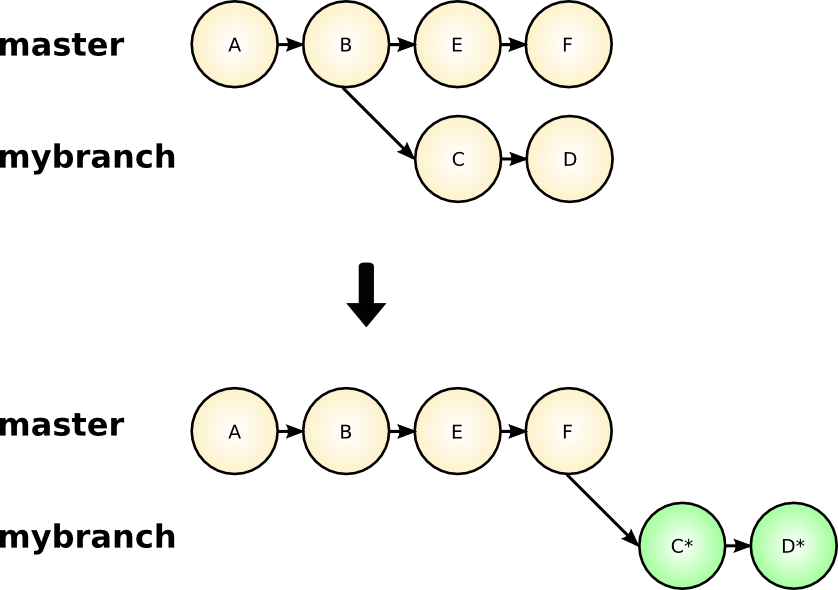
\includegraphics[width=1.0\textwidth]{images/git-rebase.png}
  \end{center}

\end{frame}

%%%%%%%%%%%%%%%%%%%%

\begin{frame}
  \frametitle{Merge two branches}

  \begin{center}
    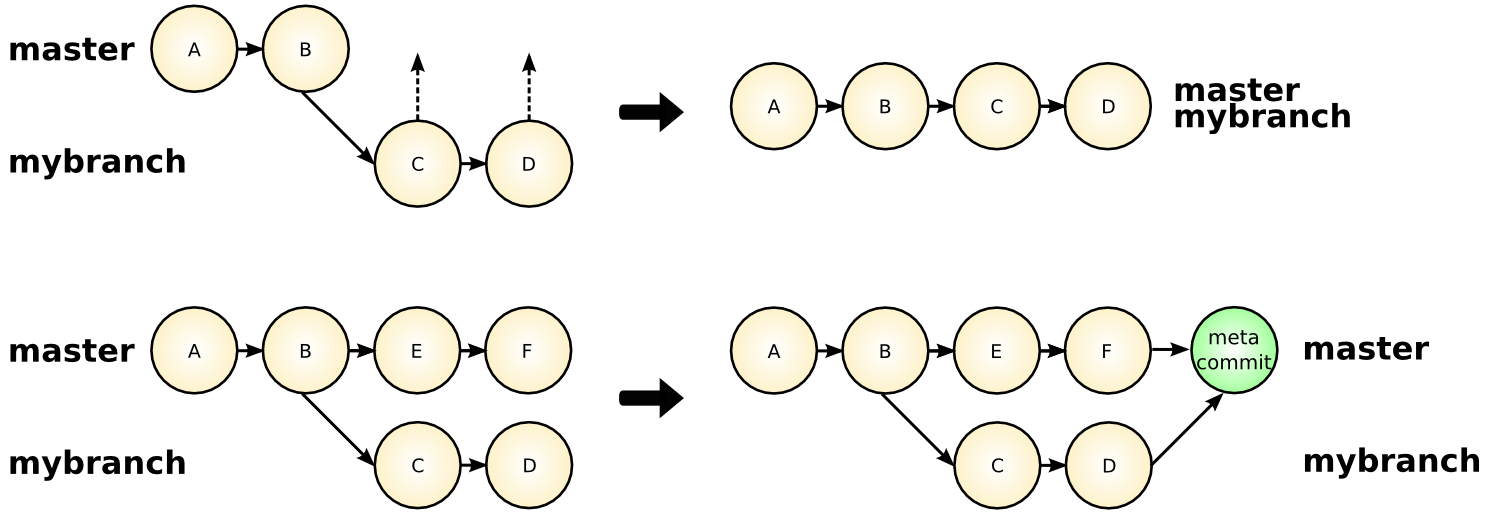
\includegraphics[width=1.0\textwidth]{images/git-merge.png}
  \end{center}

\end{frame}

%%%%%%%%%%%%%%%%%%%%

\begin{frame}
  \frametitle{\insertsubsection}

  \textbf{Pro tip:}\\
  \begin{itemize}
    \item Use one branch per feature/bug (contained development)
    \item Only merge with master after you're done
    \item Remember to rebase your feature branch before merging it to master
    \item Specify the origin and branch when pushing (might avoid mistakes)
    \item A good use of branches should prevent the need of \texttt{git cherry-pick}
  \end{itemize}

\end{frame}

%%%%%%%%%%%%%%%%%%%%

\begin{frame}[fragile]
  \frametitle{\insertsubsection}

\textbf{Proposed workflow:}\\

\begin{verbatim}
... [we're on master]
$ git checkout -b newfeature
... [make changes]
$ git commit -m "New feature"
$ git rebase master
$ git checkout master
$ git merge newfeature
$ git push origin master
\end{verbatim}

If push fails:\\
\begin{verbatim}
$ git pull --rebase
\end{verbatim}

\end{frame}

%%%%%%%%%%%%%%%%%%%%

\subsubsection{Working with Remote Branches}

\begin{frame}[fragile]
  \frametitle{\insertsubsubsection}

\textbf{List remote branches:}\\
\begin{verbatim}
$ git branch -r
remotes/origin/HEAD -> origin/master
remotes/origin/master
remotes/origin/newfeature
remotes/origin/newfeature2
remotes/origin/newfeature3
\end{verbatim}

\end{frame}

%%%%%%%%%%%%%%%%%%%%

\begin{frame}[fragile]
  \frametitle{\insertsubsection}

  \textbf{Push a branch to origin:}\\
\begin{verbatim}
$ git checkout newfeature
$ git push origin newfeature
\end{verbatim}

\end{frame}

%%%%%%%%%%%%%%%%%%%%

\begin{frame}[fragile]
  \frametitle{\insertsubsection}

  \textbf{Delete a remote branch in origin:}\\
\begin{verbatim}
$ git push origin :newfeature
\end{verbatim}

\end{frame}

%%%%%%%%%%%%%%%%%%%%

\begin{frame}[fragile]
  \frametitle{\insertsubsection}

  \textbf{Replace a remote branch in origin:}\\
\begin{verbatim}
$ git push origin +otherfeature:newfeature
\end{verbatim}

It's not advisable to replace branches you share with other people (it ``breaks'' other people's branch)

\end{frame}

%%%%%%%%%%%%%%%%%%%%

\subsection{git rebase -{}-interactive}

\begin{frame}
  \begin{center}
    \textbf{\Huge{\insertsubsection}}
  \end{center}
\end{frame}

%%%%%%%%%%%%%%%%%%%%

\begin{frame}
  \frametitle{\insertsubsection}

  \textbf{git rebase -{}-interactive} is a great tool that allows to:

  \begin{itemize}
    \item Meld commits together
    \item Remove commits
    \item Edit commits (it stops the rebase and allows to ammend a commit)
    \item Reorder commits
  \end{itemize}

\end{frame}

%%%%%%%%%%%%%%%%%%%%

\begin{frame}[fragile]
  \frametitle{\insertsubsection}

\begin{verbatim}
$ git rebase -i HEAD~5
\end{verbatim}

  \begin{footnotesize}
\begin{verbatim}
pick d3a7c85 New changes
pick b538761 Other changes
pick 61be62b Some nice new changes
pick e897f7f Update for release 0.9.2
pick ca33ef2 Commit that should have been in the release

# Rebase 8d9b5a1..ca33ef2 onto 8d9b5a1
#
# Commands:
#  p, pick = use commit
#  r, reword = use commit, but edit the commit message
#  e, edit = use commit, but stop for amending
#  s, squash = use commit, but meld into previous commit
\end{verbatim}
  \end{footnotesize}

\end{frame}

%%%%%%%%%%%%%%%%%%%%

\begin{frame}[fragile]
  \frametitle{\insertsubsection}

  \begin{footnotesize}
\begin{verbatim}
pick d3a7c85 New changes
squash b538761 Other changes
pick 61be62b Some nice new changes
pick ca33ef2 Commit that should have been in the release
pick e897f7f Update for release 0.9.2

# Rebase 8d9b5a1..ca33ef2 onto 8d9b5a1
#
# Commands:
#  p, pick = use commit
#  r, reword = use commit, but edit the commit message
#  e, edit = use commit, but stop for amending
#  s, squash = use commit, but meld into previous commit
\end{verbatim}
  \end{footnotesize}

\end{frame}

%%%%%%%%%%%%%%%%%%%%

\subsection{Name your stash}

\begin{frame}
  \begin{center}
    \textbf{\Huge{\insertsubsection}}
  \end{center}
\end{frame}

%%%%%%%%%%%%%%%%%%%%

\begin{frame}
  \frametitle{\insertsubsection}

  \texttt{git stash} is great for storing changes away temporarily

  \begin{itemize}
    \item Use \texttt{git stash save ``Description of changes"} so it's easy to keep track of what's what!
  \end{itemize}

\end{frame}

%%%%%%%%%%%%%%%%%%%%

\subsection{Use repos for different modules}

\begin{frame}
  \begin{center}
    \textbf{\Huge{\insertsubsection}}
  \end{center}
\end{frame}

%%%%%%%%%%%%%%%%%%%%

\begin{frame}
  \frametitle{\insertsubsection}

  Sometimes modules shouldn't be in the same repo\\

  \begin{itemize}
    \item A base + plugins project should live in different repos\\
      e.g.: GStreamer
  \end{itemize}

\end{frame}

%%%%%%%%%%%%%%%%%%%%

\subsection{Do NOT add every single file}

\begin{frame}
  \begin{center}
    \textbf{\Huge{\insertsubsection}}
  \end{center}
\end{frame}

%%%%%%%%%%%%%%%%%%%%

\begin{frame}
  \frametitle{\insertsubsection}

  Binary files, distro packages (rpms, debs) and other \textbf{auto-generated} files should not be
  included in the repo!\\Upload them somewhere else, a repo should be for source code.

\end{frame}

%%%%%%%%%%%%%%%%%%%%

\subsection{Don't break others' repos}

\begin{frame}
  \begin{center}
    \textbf{\Huge{\insertsubsection}}
  \end{center}
\end{frame}

%%%%%%%%%%%%%%%%%%%%

\begin{frame}
  \frametitle{\insertsubsection}

  Make sure that you do not change history in main branches (shared with other people)!

  \begin{itemize}
    \item Be careful when resetting and rebasing
    \item Do not force a push to a shared branch
  \end{itemize}

\end{frame}

%%%%%%%%%%%%%%%%%%%%

\subsection{Pull and rebase}

\begin{frame}
  \begin{center}
    \textbf{\Huge{\insertsubsection}}
  \end{center}
\end{frame}

%%%%%%%%%%%%%%%%%%%%

\begin{frame}
  \frametitle{\insertsubsection}

  Use \texttt{git pull -{}-rebase} in order to avoid merges from upstream commits.

\end{frame}

%%%%%%%%%%%%%%%%%%%%

\section{Other (Pro) Tips}

\begin{frame}[plain]

  \begin{center}
    \textbf{\Huge{\insertsection}}
  \end{center}

\end{frame}

%%%%%%%%%%%%%%%%%%%%

\subsection{Use git hooks to enforce standards}

\begin{frame}
  \frametitle{\insertsubsection}

  Git hooks can be used to e.g.:\\
  \begin{itemize}
    \item make sure the source honors a certain coding style
    \item force a commit message to include a bug tracker reference
    \item etc.
  \end{itemize}

\end{frame}

%%%%%%%%%%%%%%%%%%%%

\subsection{git clean}

\begin{frame}
  \frametitle{\insertsubsection}

  \begin{center}
    \textbf{Be careful with git clean!}
  \end{center}

  \texttt{git clean -xdf} will really delete things, no reflog, no nothing!\\
  \textbf{Always dry-run first!}\\
  \texttt{\$ git clean -nxdf}

\end{frame}

%%%%%%%%%%%%%%%%%%%%

\subsection{Use command aliases and auto-completion}

\begin{frame}
  \frametitle{\insertsubsection}

  Use git aliases and auto-completion for extra productivity:\\
  \begin{itemize}
      \item \texttt{git config -{}-global alias.ci 'commit'}
      \item \texttt{git config -{}-global alias.co 'checkout'}
      \item \texttt{git config -{}-global alias.st 'status'}
  \end{itemize}
\vspace*{20pt}
  Auto-completion:\\
  \texttt{http://code-worrier.com/blog/autocomplete-git/}

\end{frame}

%%%%%%%%%%%%%%%%%%%%

\subsection{Show your HEAD in shell's prompt}

\begin{frame}
  \frametitle{\insertsubsection}

  Change your shell's prompt to show your git branch:\\
  \texttt{\footnotesize http://code-worrier.com/blog/git-branch-in-bash-prompt/}

  \vspace*{20pt}
  \begin{footnotesize}
    \texttt{[17:42][\textasciitilde{}/presentations/git-best-practices{\color{myblue}\textbf{(master)}}]\$}
  \end{footnotesize}

\end{frame}

%%%%%%%%%%%%%%%%%%%%

\subsection{Do NOT copy/paste diffs}

\begin{frame}[fragile]
  \frametitle{\insertsubsection}

  Create patches by using \texttt{git format-patch}

  \begin{itemize}
    \item Patches of the last 2 commits:
\begin{verbatim}
$ git format-patch HEAD~2
0001-Some-nice-changes.patch
0002-Some-other-nice-changes.patch
\end{verbatim}
  \end{itemize}

  You can even send them by email from git using \texttt{git send-email}!

\end{frame}

%%%%%%%%%%%%%%%%%%%%

\subsection{See what your tree looks like}

\begin{frame}
  \frametitle{\insertsubsection}

  Having a global picture of your tree is important!\\
  \vspace{20pt}

  Use \texttt{git lola}:\\

  \begin{footnotesize}
    \texttt{git config -{}-global alias.lola "log -{}-graph -{}-decorate -{}-pretty=oneline -{}-abbrev-commit -{}-all"}
  \end{footnotesize}

  \vspace{20pt}
  ... or use \texttt{tig} for an interactive CLI viewer

  \vspace{20pt}
  ... or use or a graphical tool like \textit{gitg}

\end{frame}

%%%%%%%%%%%%%%%%%%%%

\begin{frame}[plain]
%  \frametitle{\insertsubsection}

  \begin{center}
    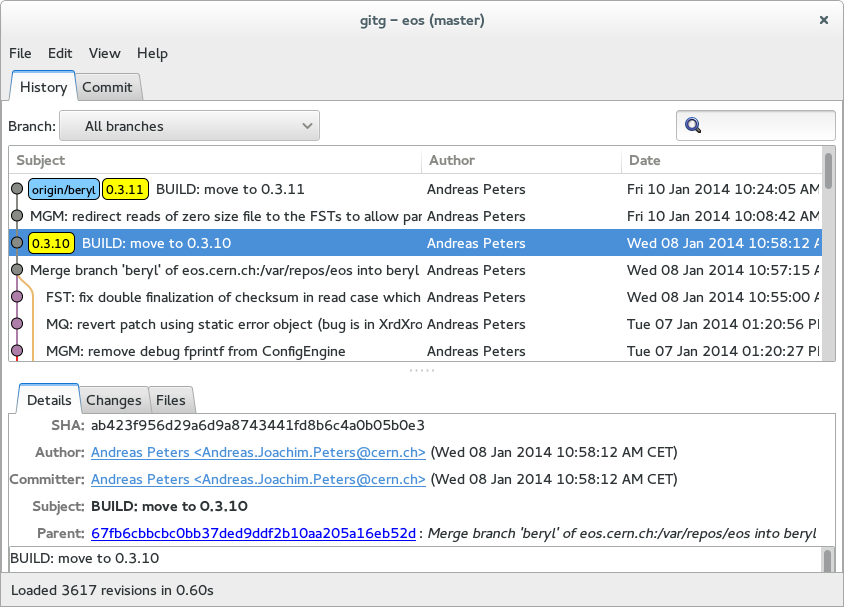
\includegraphics[width=1.0\textwidth]{images/gitg.png}
  \end{center}
\end{frame}

%%%%%%%%%%%%%%%%%%%%

\section{Credits}

\begin{frame}

  \vspace{60pt}
  \begin{center}
    \Huge{\textbf{Thank you!}}
  \end{center}

  \vspace{60pt}
  \begin{scriptsize}
    \begin{itemize}
      \item Git's logo, CC by Jason Long
      \item Linus Torvalds picture, CC by The Linux Foundation
      \item Kid picture, CC by Juhan Sonin
      \item Monkey picture, CC by Scott Monty
      \item Slides and diagrams based in \\\textit{Git: The Stupid Content Tracker} by Mario Sánchez Prada
    \end{itemize}
  \end{scriptsize}

\end{frame}

%%%%%%%%%%%%%%%%%%%%

